\section{Pong Soup and Labyrinth Learning curves}
\label{sec:appendix_extra_curves}


We include training curves for all Pong variants and Labyrinth games we considered.
The plots show how two-column progressive networks perform as compared to Baseline 3 (gray dashed line), a model pretrained on the \textit{source} game and then finetuned on the particular \textit{target} game, and Baseline 1 (black dotted line), where a single column is trained on the \textit{source} game.

\begin{sidewaystable}
     \begin{tabular}{m{.05\textwidth} >{\centering}m{.22\textwidth} >{\centering}m{.22\textwidth} >{\centering}m{.22\textwidth} >{\centering\arraybackslash}m{.22\textwidth} }
	Source & Target: Pong & Target: Black & Target: H-flip & Target: HV-flip \\
     	
	Pong &
        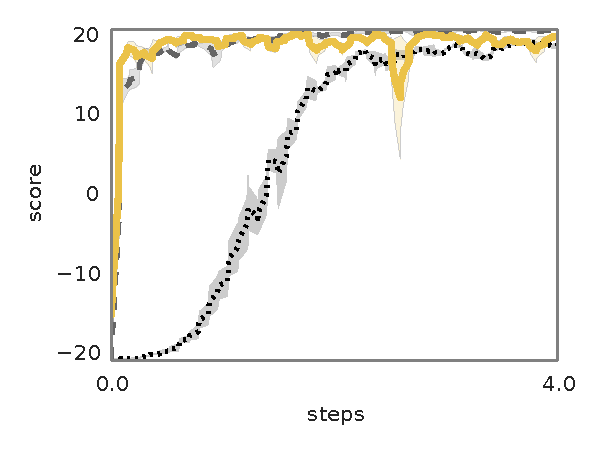
\includegraphics[width=.22\textwidth]{figures/app_plots/pongs/pong/pong} &
        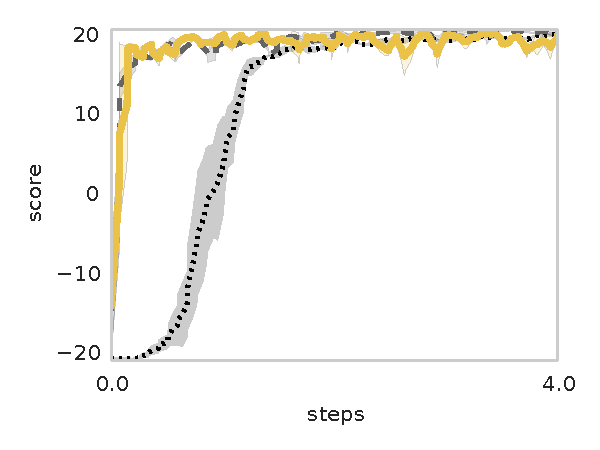
\includegraphics[width=.22\textwidth]{figures/app_plots/pongs/pong/pong_black} &
        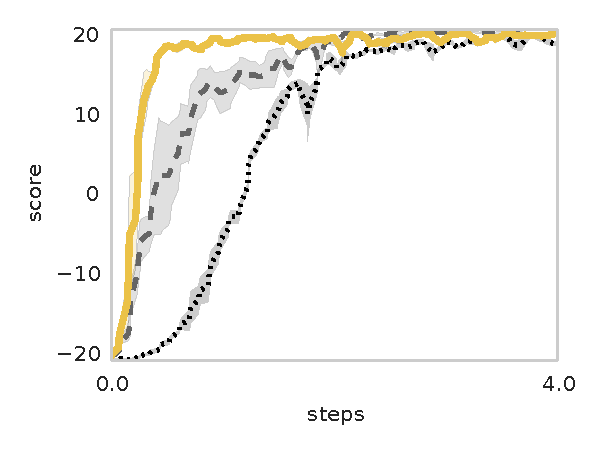
\includegraphics[width=.22\textwidth]{figures/app_plots/pongs/pong/pong_h_flip} &
        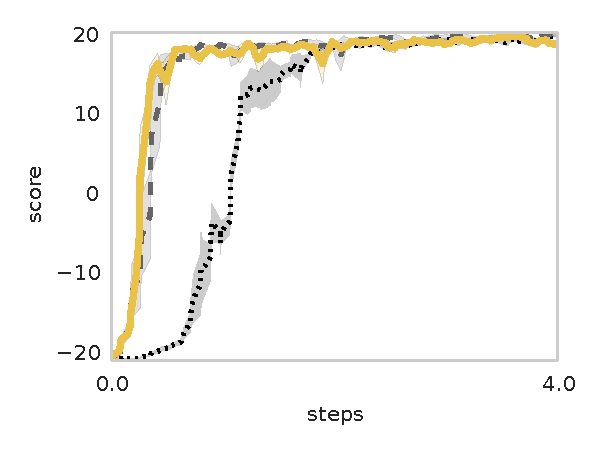
\includegraphics[width=.22\textwidth]{figures/app_plots/pongs/pong/pong_hv_flip} \\

	Noisy &
	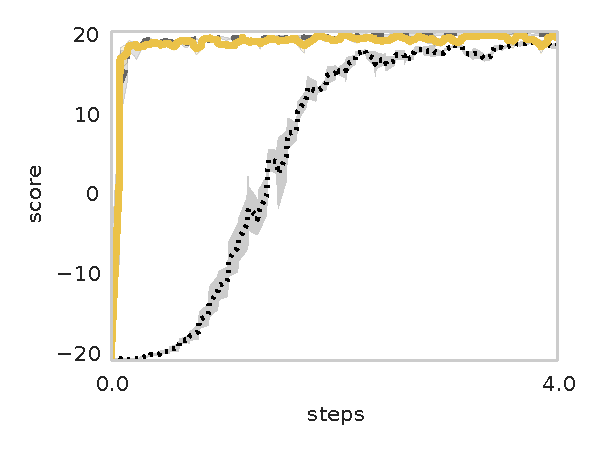
\includegraphics[width=.22\textwidth]{figures/app_plots/pongs/pong_noise/pong} &
        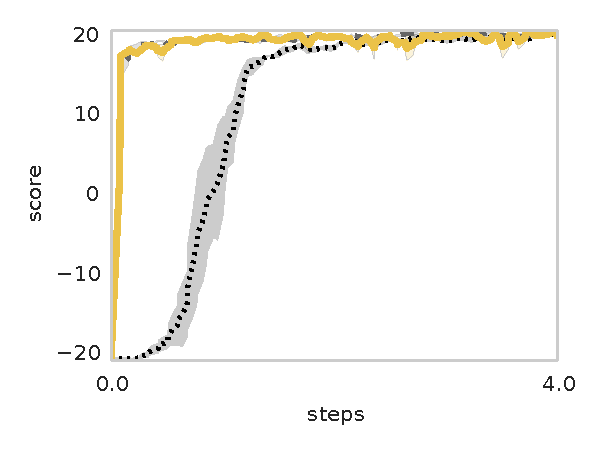
\includegraphics[width=.22\textwidth]{figures/app_plots/pongs/pong_noise/pong_black} &
        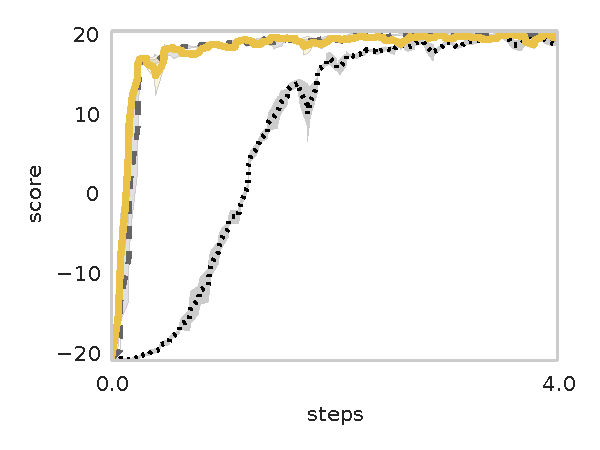
\includegraphics[width=.22\textwidth]{figures/app_plots/pongs/pong_noise/pong_h_flip} &
        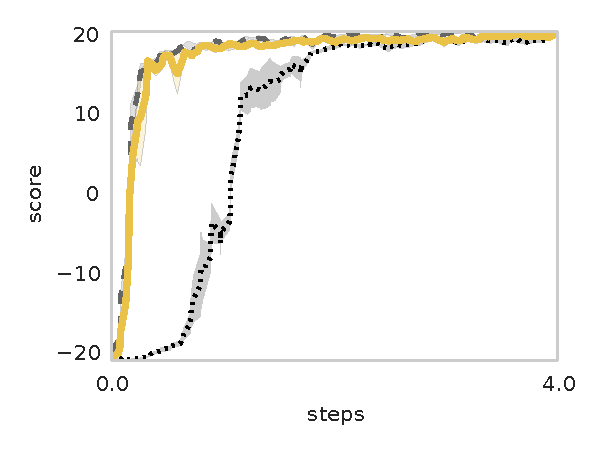
\includegraphics[width=.22\textwidth]{figures/app_plots/pongs/pong_noise/pong_hv_flip} \\

	H-flip &
	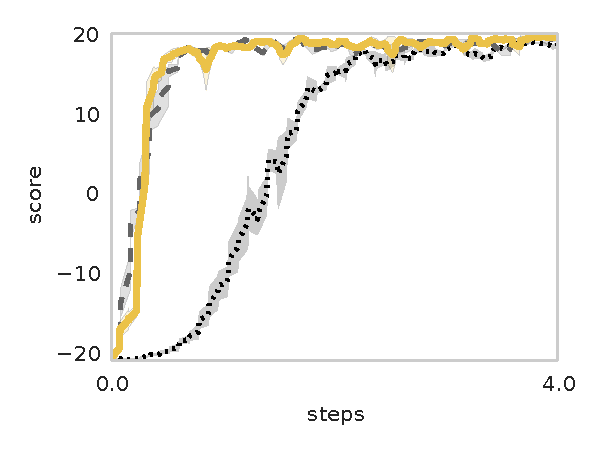
\includegraphics[width=.22\textwidth]{figures/app_plots/pongs/pong_h_flip/pong} &
        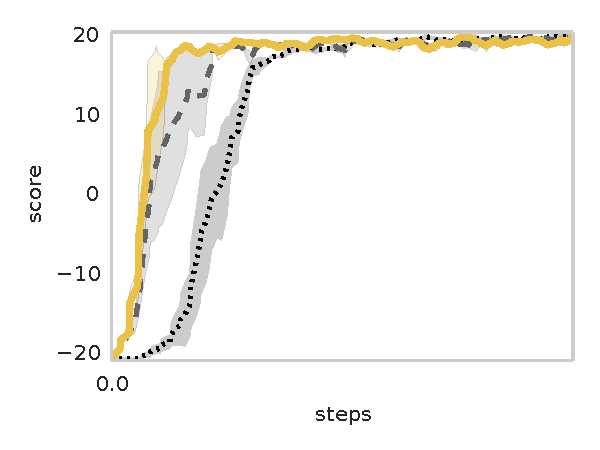
\includegraphics[width=.22\textwidth]{figures/app_plots/pongs/pong_h_flip/pong_black} &
        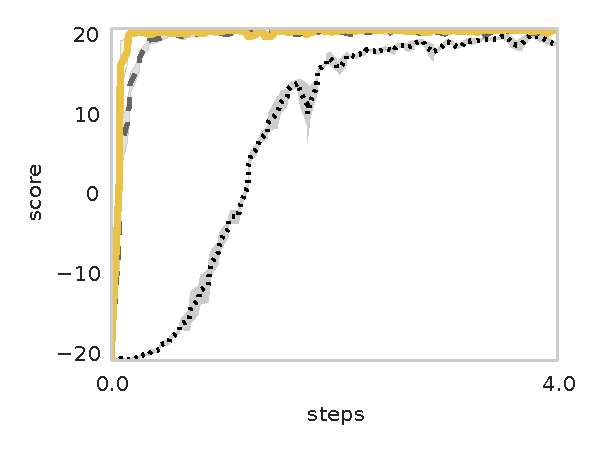
\includegraphics[width=.22\textwidth]{figures/app_plots/pongs/pong_h_flip/pong_h_flip} &
        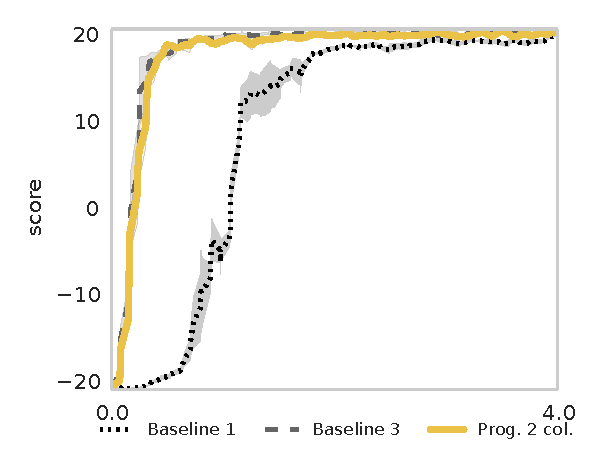
\includegraphics[width=.22\textwidth]{figures/app_plots/pongs_legend/pong_h_flip/pong_hv_flip} \\
    \end{tabular}
\end{sidewaystable}



\begin{sidewaystable}
     \begin{tabular}{m{.05\textwidth} >{\centering}m{.22\textwidth} >{\centering}m{.22\textwidth} >{\centering}m{.22\textwidth} >{\centering\arraybackslash}m{.22\textwidth} }
	Source & Target: Noisy & Target: V-flip & Target: White & Target: Zoom \\
     	
	Pong &
        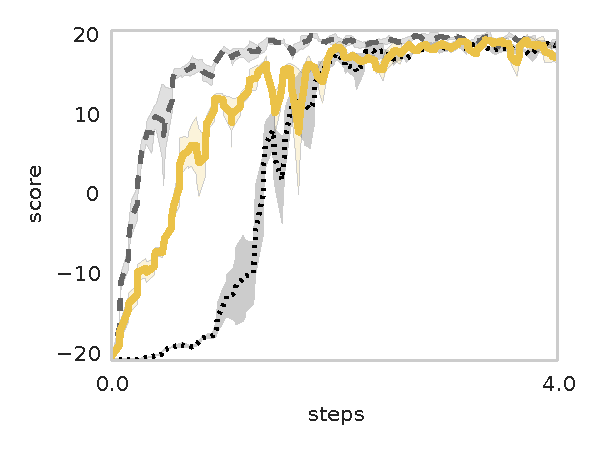
\includegraphics[width=.22\textwidth]{figures/app_plots/pongs/pong/pong_noise} &
        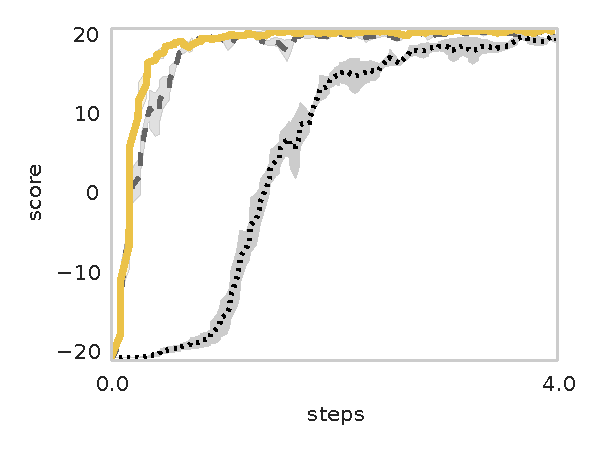
\includegraphics[width=.22\textwidth]{figures/app_plots/pongs/pong/pong_v_flip} &
        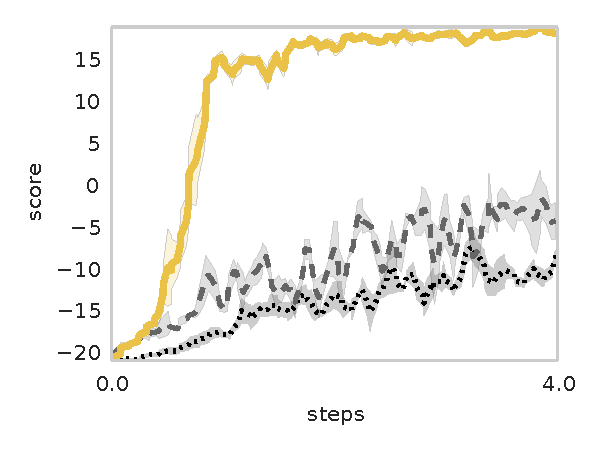
\includegraphics[width=.22\textwidth]{figures/app_plots/pongs/pong/pong_white} &
        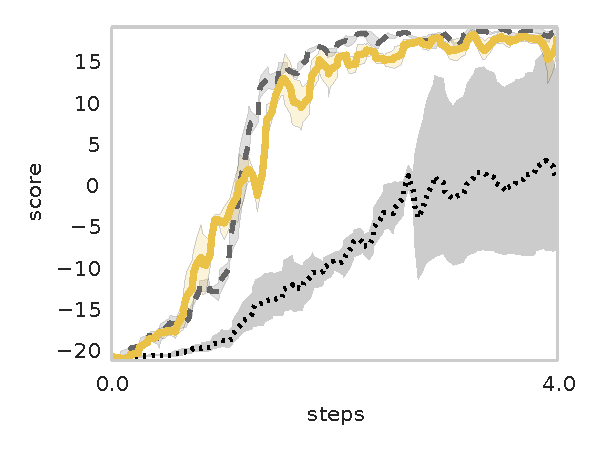
\includegraphics[width=.22\textwidth]{figures/app_plots/pongs/pong/pong_zoom} \\

	Noisy &
        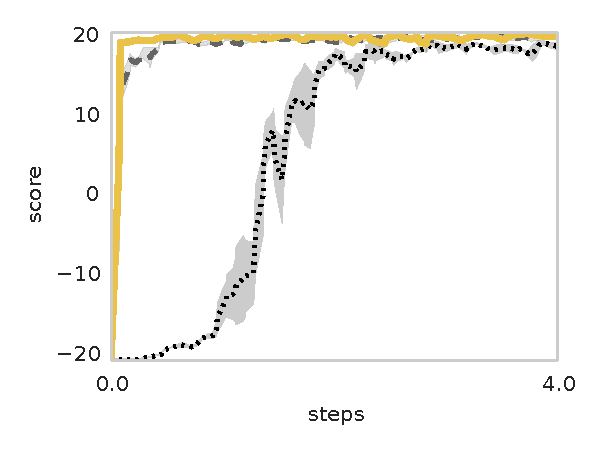
\includegraphics[width=.22\textwidth]{figures/app_plots/pongs/pong_noise/pong_noise} &
        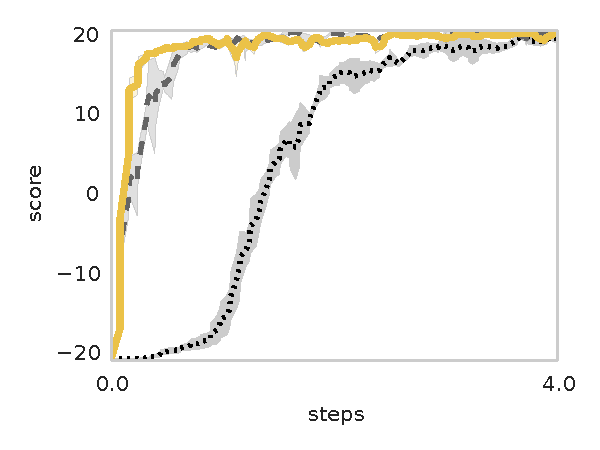
\includegraphics[width=.22\textwidth]{figures/app_plots/pongs/pong_noise/pong_v_flip} &
        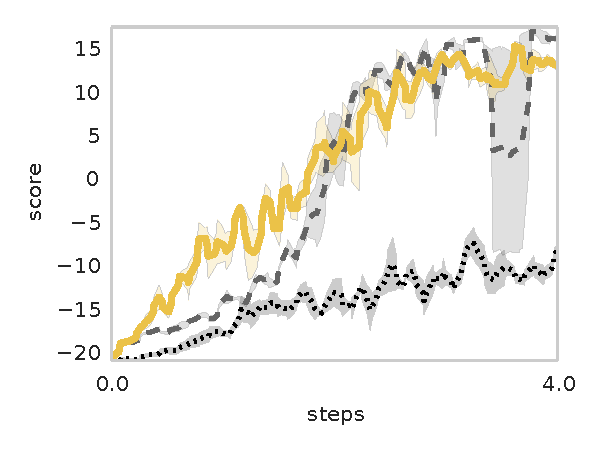
\includegraphics[width=.22\textwidth]{figures/app_plots/pongs/pong_noise/pong_white} &
        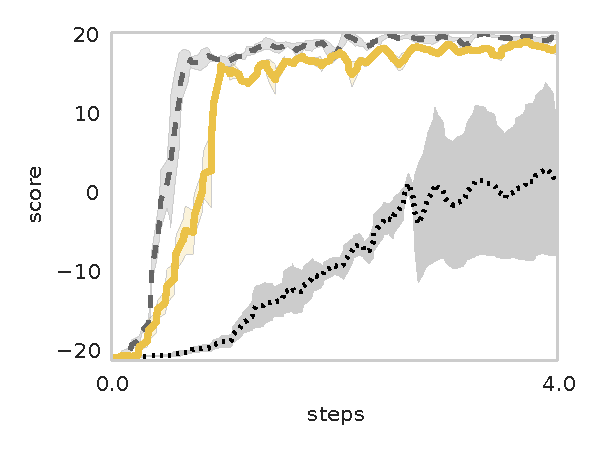
\includegraphics[width=.22\textwidth]{figures/app_plots/pongs/pong_noise/pong_zoom} \\

	H-flip &
        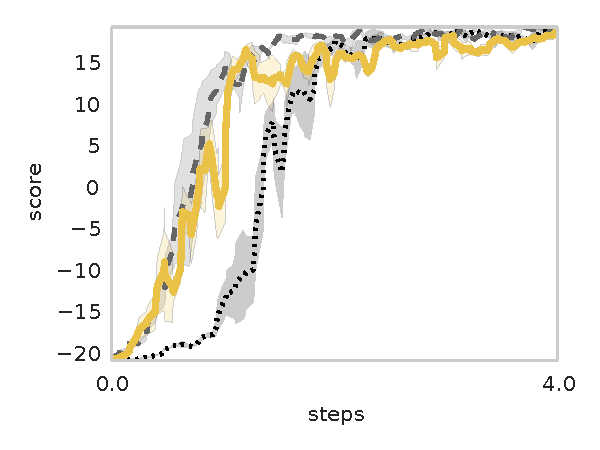
\includegraphics[width=.22\textwidth]{figures/app_plots/pongs/pong_h_flip/pong_noise} &
        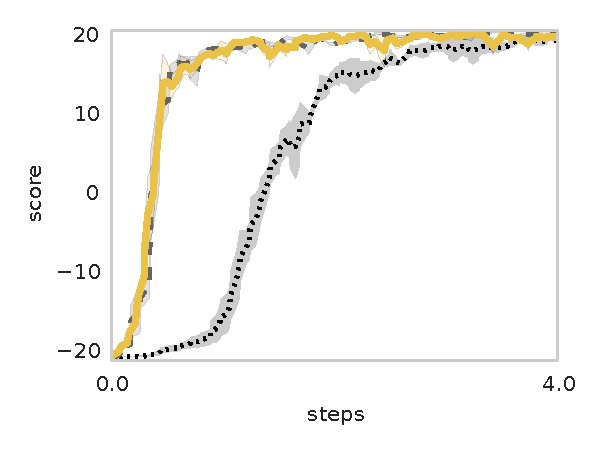
\includegraphics[width=.22\textwidth]{figures/app_plots/pongs/pong_h_flip/pong_v_flip} &
        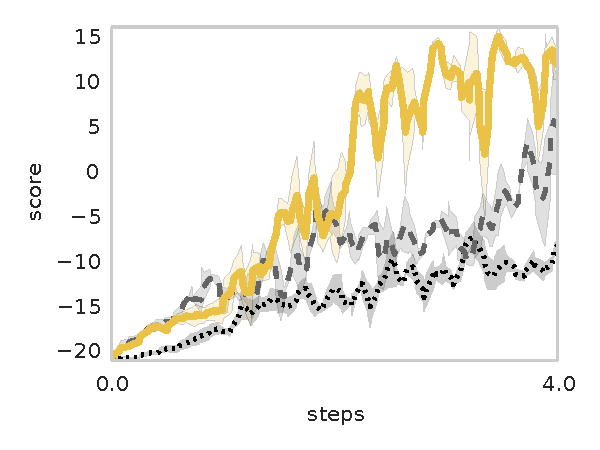
\includegraphics[width=.22\textwidth]{figures/app_plots/pongs/pong_h_flip/pong_white} &
        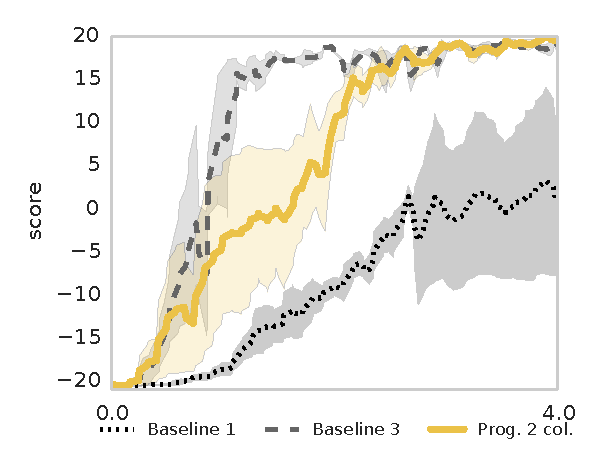
\includegraphics[width=.22\textwidth]{figures/app_plots/pongs_legend/pong_h_flip/pong_zoom} \\
    \end{tabular}
\end{sidewaystable}





\begin{sidewaystable}
     \begin{tabular}{m{.05\textwidth} >{\centering}m{.22\textwidth} >{\centering}m{.22\textwidth} >{\centering}m{.22\textwidth} >{\centering\arraybackslash}m{.22\textwidth} }
	Source & Target: Track 1 & Target: Track 2 & Target: Track 3 & Target: Track 4  \\
     	
	Avoid 1 &
        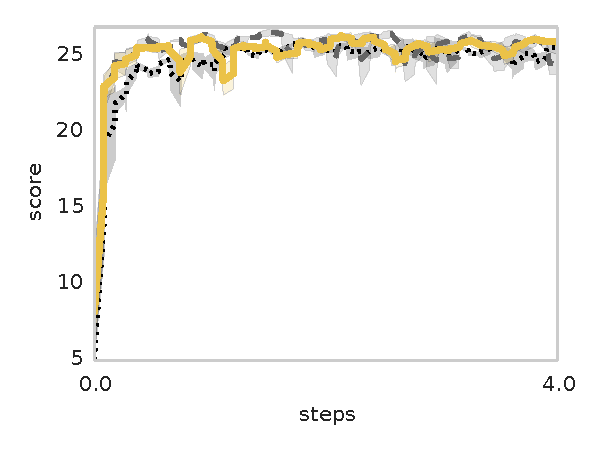
\includegraphics[width=.22\textwidth]{figures/app_plots/lab/sa1/seek_track_01} &
        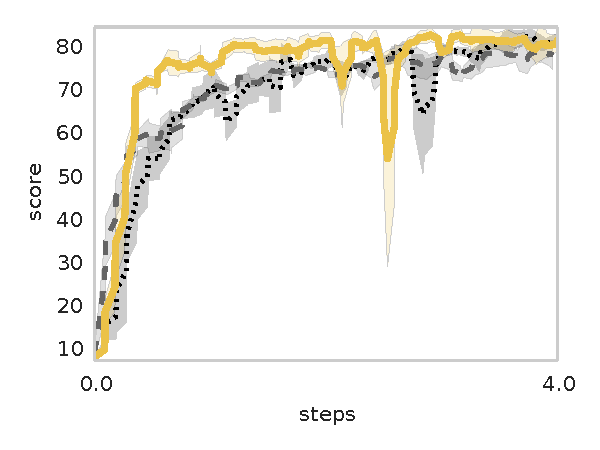
\includegraphics[width=.22\textwidth]{figures/app_plots/lab/sa1/seek_track_02} &
        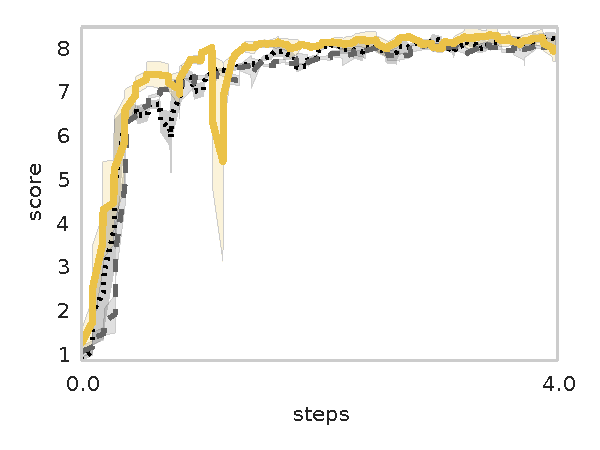
\includegraphics[width=.22\textwidth]{figures/app_plots/lab/sa1/seek_track_03} &
        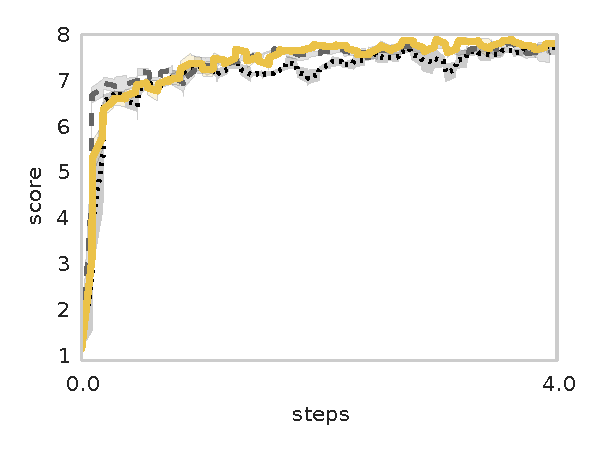
\includegraphics[width=.22\textwidth]{figures/app_plots/lab/sa1/seek_track_04} \\

	Track 1 &
        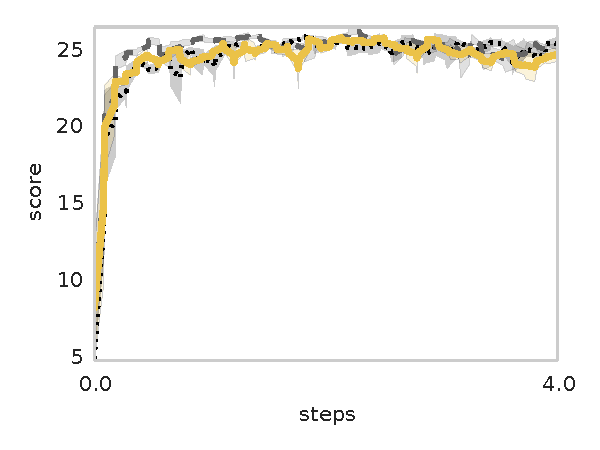
\includegraphics[width=.22\textwidth]{figures/app_plots/lab/st1/seek_track_01} &
        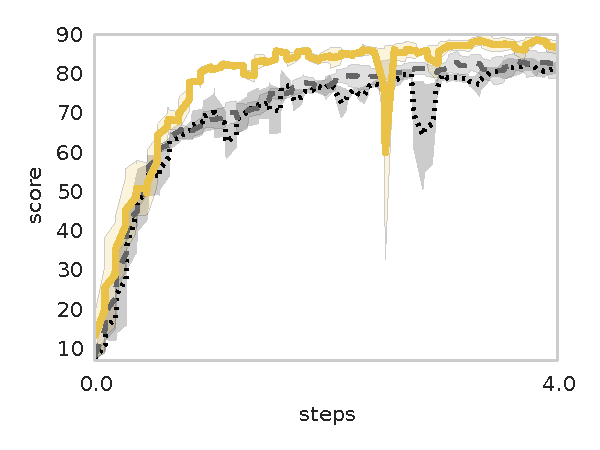
\includegraphics[width=.22\textwidth]{figures/app_plots/lab/st1/seek_track_02} &
        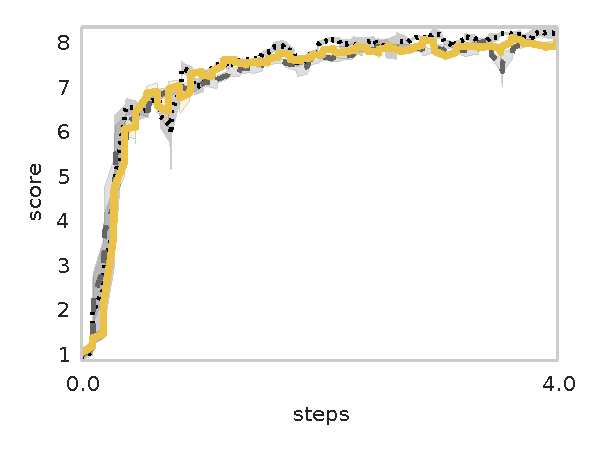
\includegraphics[width=.22\textwidth]{figures/app_plots/lab/st1/seek_track_03} &
        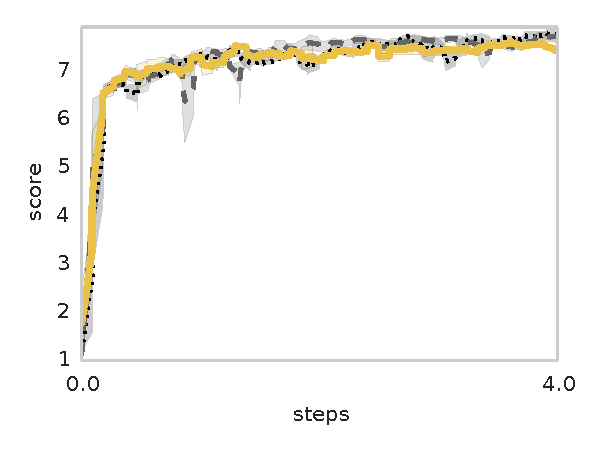
\includegraphics[width=.22\textwidth]{figures/app_plots/lab/st1/seek_track_04} \\

	Maze Y &
        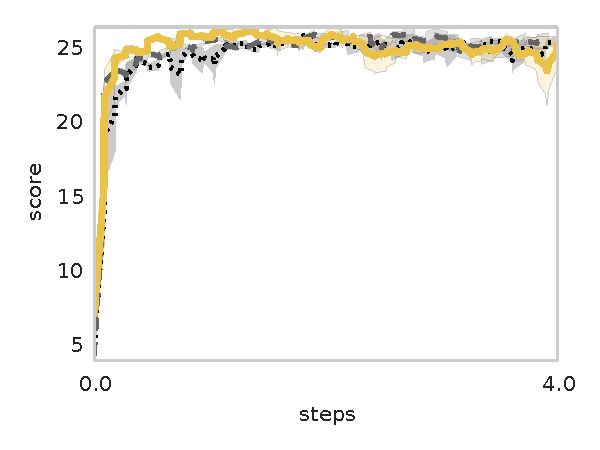
\includegraphics[width=.22\textwidth]{figures/app_plots/lab/smy1/seek_track_01} &
        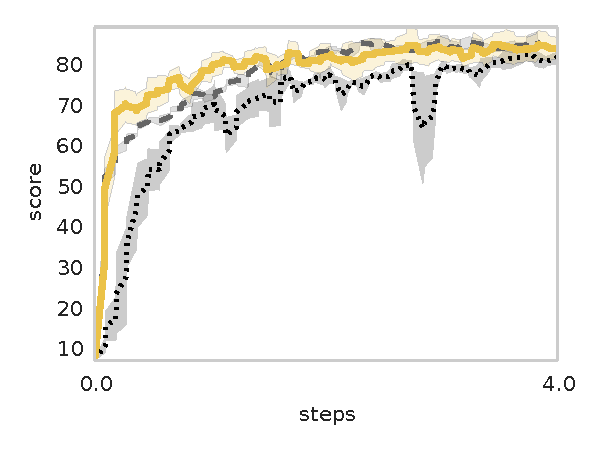
\includegraphics[width=.22\textwidth]{figures/app_plots/lab/smy1/seek_track_02} &
        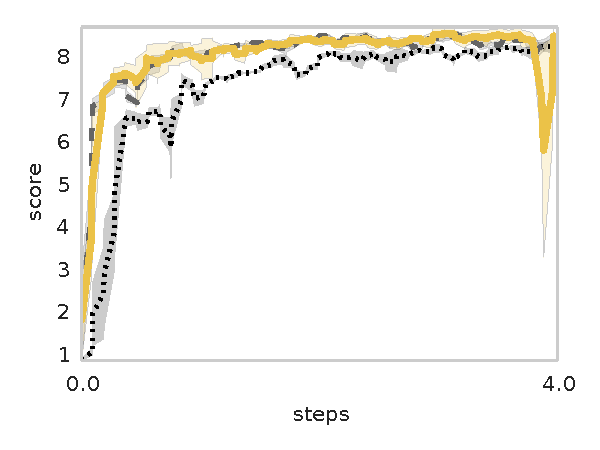
\includegraphics[width=.22\textwidth]{figures/app_plots/lab/smy1/seek_track_03} &
        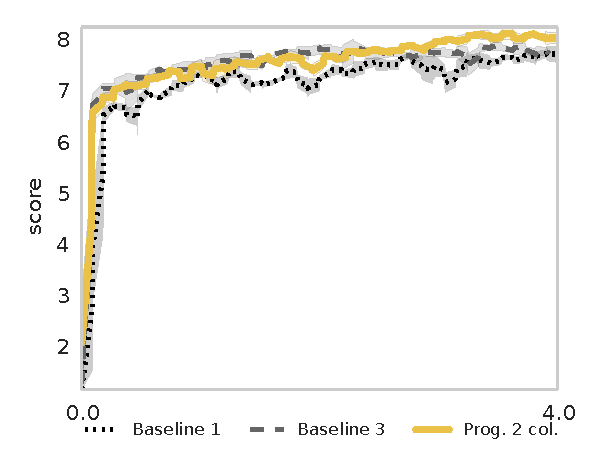
\includegraphics[width=.22\textwidth]{figures/app_plots/lab_legend/smy1/seek_track_04} \\
    \end{tabular}
\end{sidewaystable}


\begin{sidewaystable}
     \begin{tabular}{m{.05\textwidth} >{\centering}m{.22\textwidth} >{\centering}m{.22\textwidth} >{\centering}m{.22\textwidth} >{\centering\arraybackslash}m{.22\textwidth} }
	Source & Target: Avoid 1 & Target: Avoid 2 & Target: Maze Y & Target: Maze M \\
     	
	Avoid 1 &
        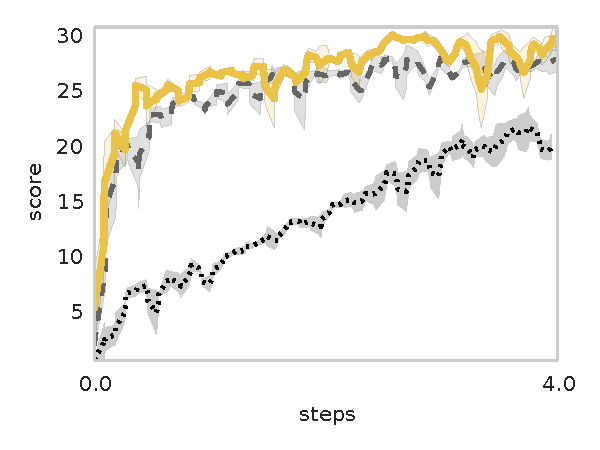
\includegraphics[width=.22\textwidth]{figures/app_plots/lab/sa1/seekavoid_arena_01} &
        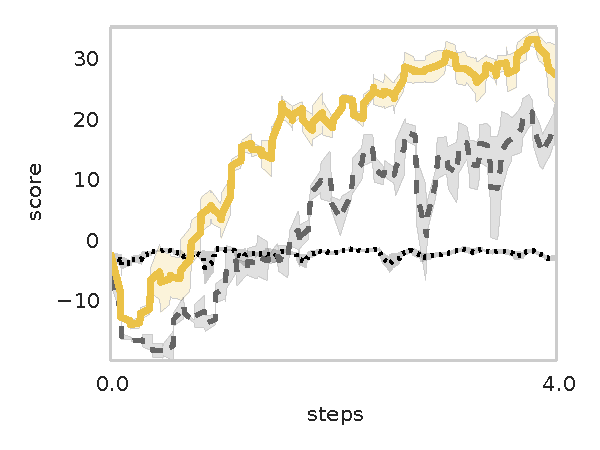
\includegraphics[width=.22\textwidth]{figures/app_plots/lab/sa1/seekavoid_arena_02} &
        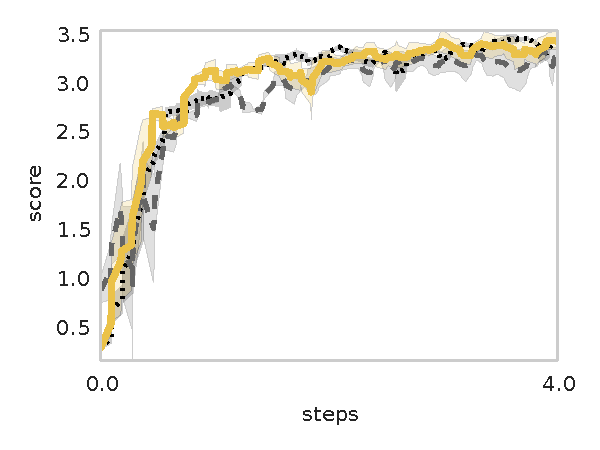
\includegraphics[width=.22\textwidth]{figures/app_plots/lab/sa1/seek_maze_y_01} &
        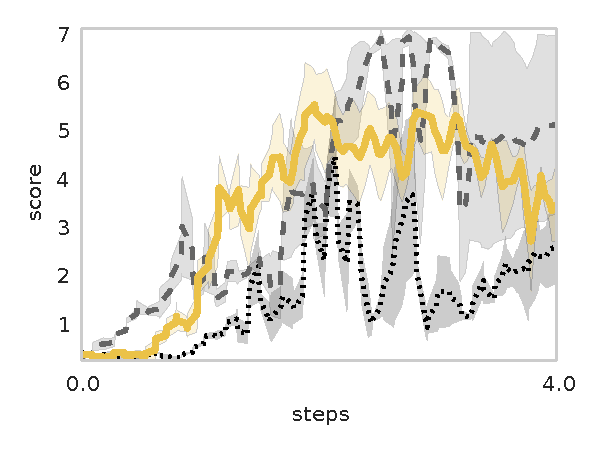
\includegraphics[width=.22\textwidth]{figures/app_plots/lab/sa1/seek_maze_m_01} \\

	Track 1 &
        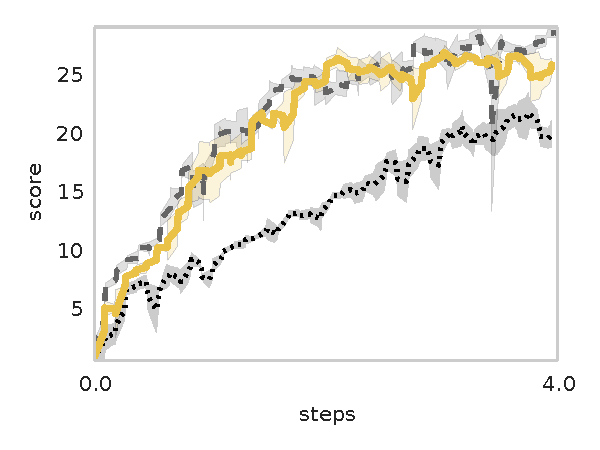
\includegraphics[width=.22\textwidth]{figures/app_plots/lab/st1/seekavoid_arena_01} &
        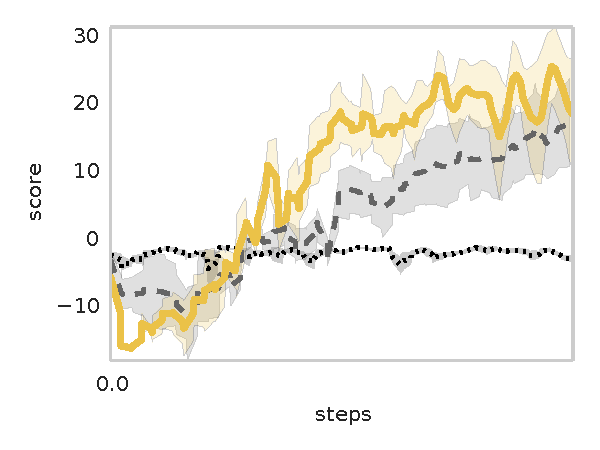
\includegraphics[width=.22\textwidth]{figures/app_plots/lab/st1/seekavoid_arena_02} &
        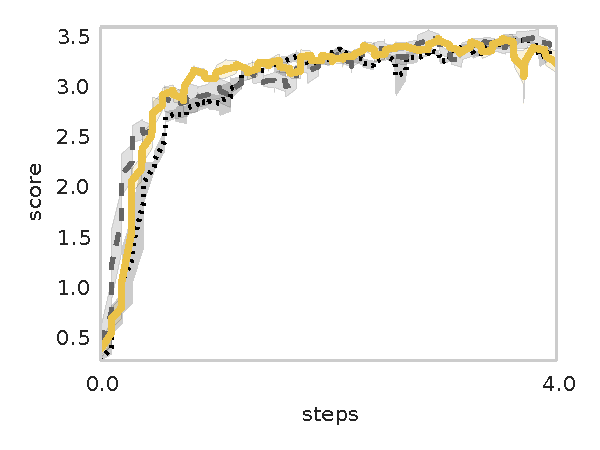
\includegraphics[width=.22\textwidth]{figures/app_plots/lab/st1/seek_maze_y_01} &
        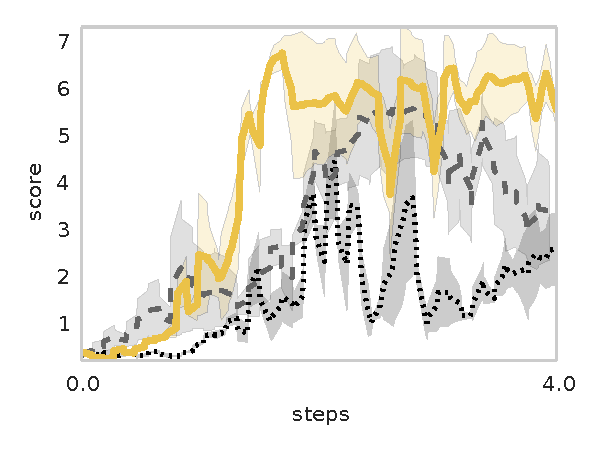
\includegraphics[width=.22\textwidth]{figures/app_plots/lab/st1/seek_maze_m_01} \\

	Maze Y &
        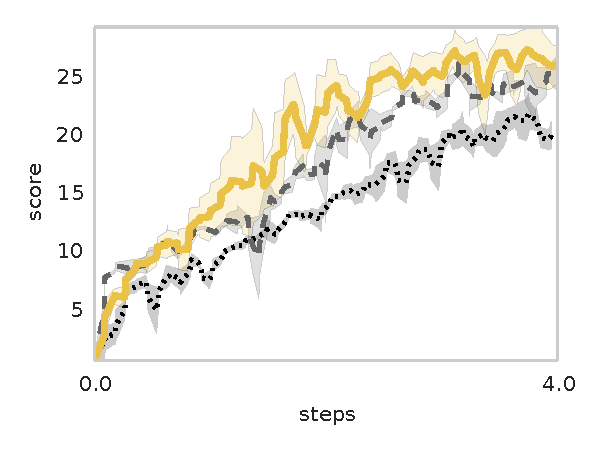
\includegraphics[width=.22\textwidth]{figures/app_plots/lab/smy1/seekavoid_arena_01} &
        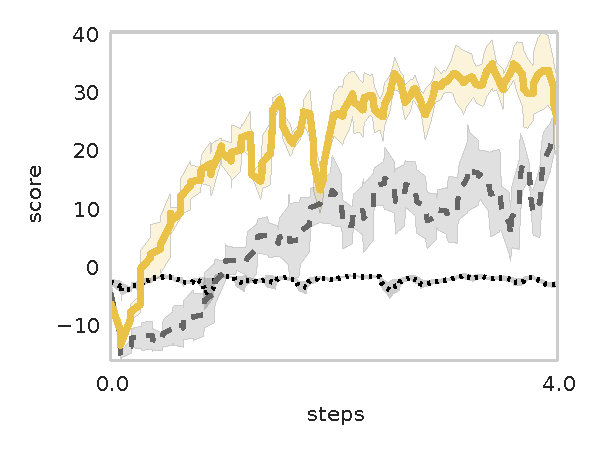
\includegraphics[width=.22\textwidth]{figures/app_plots/lab/smy1/seekavoid_arena_02} &
        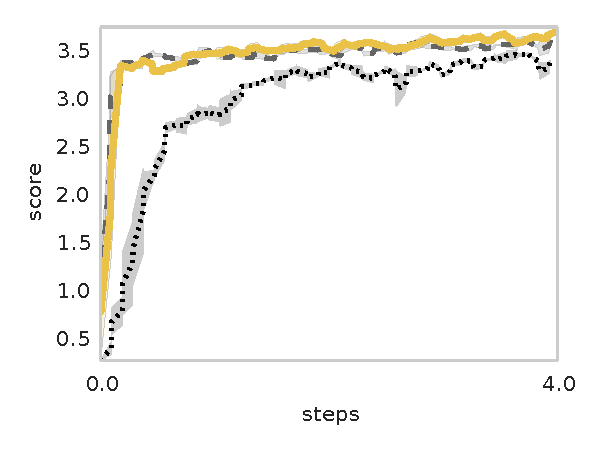
\includegraphics[width=.22\textwidth]{figures/app_plots/lab/smy1/seek_maze_y_01} &
        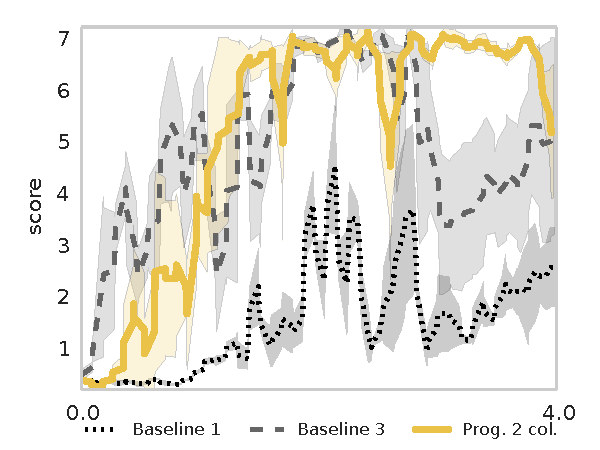
\includegraphics[width=.22\textwidth]{figures/app_plots/lab_legend/smy1/seek_maze_m_01} \\
    \end{tabular}
\end{sidewaystable}
